\subsection{Long-Slit Spectroscopy in L/M- and N-bands}\label{lss:overview}
\subsubsection{The workflow cascades}\label{lss:cascade_overview}
The purpose of these workflows is to correct or remove contributions from
the instrument, telescope, and atmosphere and generate science-grade
data products for the L/M- and N-band \ac{LSS}
mode. Since the Geosnap detector is still under investigation, we currently assume basically the same reduction cascade for both spectral ranges LM and N, respectively. The major differences at the time being are the subtraction methods for the sky background (nodding in LM, chop-nodding in N band) and the absence of \ac{WCU} laser sources in the N-band, which are only available during \ac{AIT} phase to generate a first guess of the pixel-to-wavelength relation. Therefore the first guess wavelength solution in the N-band will be based on that \ac{AIT} data. As we assume the instrument to be very stable, that approach should be sufficient for the low-resolution N-band spectroscopy. In the LM range, two fixed-frequency lasers ($@3.39$µm and $@5.26$µm) and one tuneable ($4.68....4.78$µm) is foreseen in the \ac{WCU} to be taken on daily basis (cf. \cite{METIS-calibration_plan}). Although mainly foreseen to be used for the high-resolution spectroscopy \ac{IFU} mode, we can use these laser sources for the LM-band \ac{LSS} as well.

Special emphasis has to be drawn to the effects of the Earth's atmosphere in several respects:
\begin{itemize}
\item Wavelength calibration: Absorption/emission features are intended to be
  used for the wavelength calibration. Thus, a good knowledge on /
  identification of these features is crucial for the accuracy of the
  wavelength calibration.
\item Telluric correction: In the MIR regime telluric absorption is -among others- one of the most dominant effects visible in    
 spectra. Modelling approaches like \texttt{molecfit} heavily rely on accurate atmospheric input profiles, which represent the actual state and composition of the Earth's atmosphere. This especially applies to the \ac{PWV} content since this is the most dominant and most variable species. We also include the classical approach for the telluric correction (i.e. deriving the Earth's atmosphere transmission by means of standard stars) to be able to achieve a good removal of sky emission in case \texttt{molecfit} appears to be insufficient.
\item Atmospheric dispersion: \ac{METIS} will have \ac{ADC}s compensating the effect of atmospheric dispersion. However, for technical reasons these ADCs are fixed at several positions. This means that the     compensation is only partially, leading to two practical effects:
  (a) wavelength-dependent slit losses, and (b) distortions in both,
  the spatial and the spectral direction (see \cite{METIS-ADC_study}
  for more details). For both, the pipeline needs to correct
  for. It is foreseen to determine these slitlosses on yearly basis with a separate calibration task (cf. \cite{METIS-calibration_plan}) and create a slit-loss table to be included in the static calibration database.
\end{itemize}

%However, to keep flexibility and independence of both branches, we
%define different recipes for the time being, although they will be
%mostly based on the same algorithms. We therefore focus here on the LM-band only.

Figures~\ref{Fig:LMLssAssomap1} and \ref{Fig:LMLssAssomap2} show the reduction cascade and the association map for the recipes handling L/M-long-slit
spectroscopy data.  %Tables~\ref{Tab:LMLssDatProc1} and ~\ref{Tab:LMLssDatProc2} contain the data processing table for this mode. For the N-band \ac{LSS} mode the cascade and the data processing table is given in Figs. \ref{Fig:NLssAssomap1} and \ref{Fig:NLssAssomap2} and Tables~\ref{Tab:NLssDatProc1} and ~\ref{Tab:NLssDatProc2}, respectively (cf. also Fig.~\ref{Fig:LSScascadelegend}).

In general, there are four major steps in each of the two cascades:
\begin{itemize}
    \item \textbf{Preparation steps:} This part contains the recipes, which are invoked only rarely, e.g. after major instrument interventions, or on monthly/yearly basis to update the static calibration database. These recipes are therefore not shown in the cascade in Figs.~\ref{Fig:LMLssAssomap1}/\ref{Fig:LMLssAssomap2} and \ref{Fig:NLssAssomap1}/\ref{Fig:NLssAssomap2} and the corresponding data processing tables. In case of the \ac{LSS} pipeline this concerns the creation of the gain maps/linearity checks (see Section~\ref{sssec:metis_det_lingain}), the determination of the slit losses induced by the fixed positions of the ADCs (cf. Section~\ref{sssec:adc_slitlosses} and Section "Calibration of slit losses" in Calibration plan \cite{METIS-calibration_plan}) and the zero position of the chopping mirror (see Section~\ref{ssec:metisimgchophome} and Section "Chopper Home Position" in \cite{METIS-calibration_plan} for more details). 
    \item \textbf{Basic steps}: The basic steps aim for correcting the detector influence, in particular the dark correction and the determination of the master \ac{RSRF}. Special cases are the linearity correction and (optionally) the persistence subtraction, which are done consecutively in the individual recipes as first two reduction steps on the corresponding raw data. %The basic function for that will be provided by \ac{ESO}\footnote{c.f. \ac{ELT} working group on detectors/persistence} and is not a dedicated recipe. 
    \item \textbf{Calibration/correction steps}: This is the main part which incorporates the order trace detection, distortion, wavelength and absolute flux calibration. In case a dedicated \ac{STD} star is provided, a transmission curve is created for the telluric correction.
    \item \textbf{Post-calibration steps}: After having calibrated spectra at hand, the last step is the telluric absorption correction with \texttt{molecfit}. This is optional in case the user decided not to use the classic approach with a standard star.
\end{itemize}

\begin{figure}[ht]
  \centering
  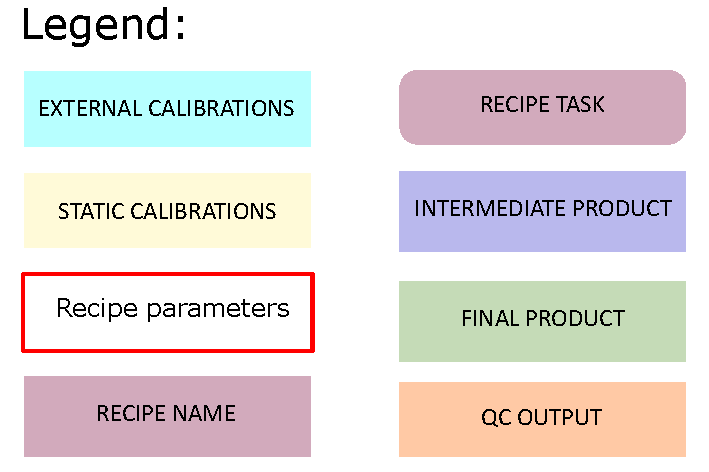
\includegraphics[width=0.4\textheight]{figures/legend.pdf}
  \caption[Legend]{Legend of the coloured boxes in the \ac{LSS} cascades.}
  \label{Fig:LSScascadelegend}
\end{figure}
\clearpage

\newgeometry{bottom=0.5cm, right=0.1cm, left=0.1cm}
% This geometry makes the tables/figures fit, but messes up the header a bit.

\begin{landscape}
\begin{figure}[ht]
  \centering
  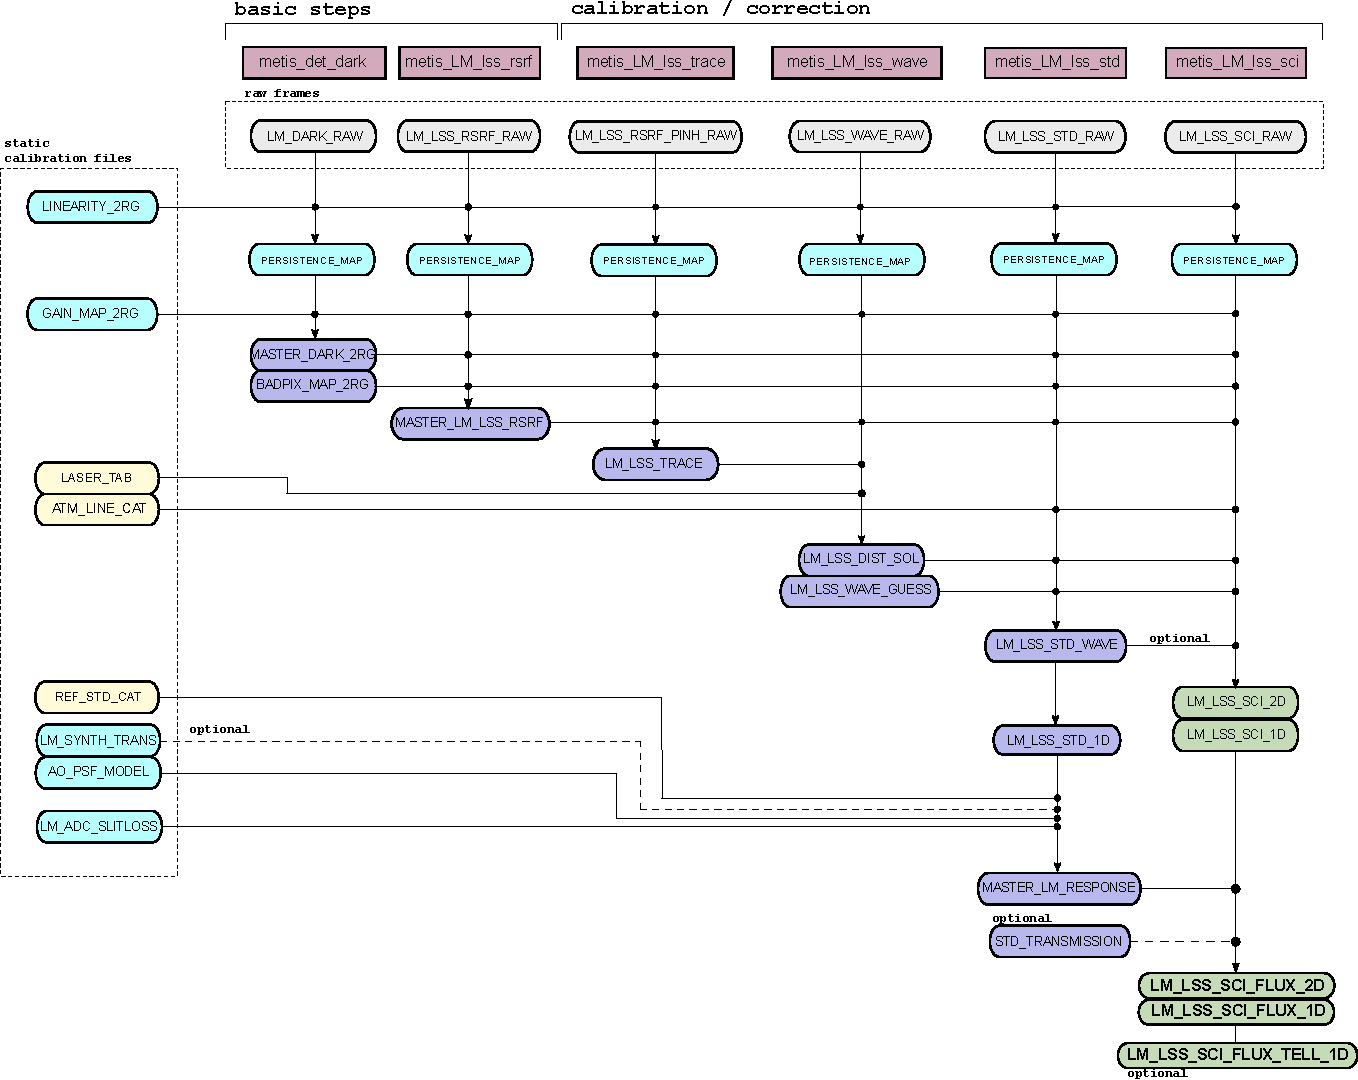
\includegraphics{figures/LM_LSS_pipeline_wf_draft_latest_part_1_v0.83.pdf}
  \caption[Reduction cascade and association map for LM long-slit
  spectroscopy]{Part 1 of the reduction cascade and association map for long-slit
    spectroscopy in the LM bands.}
  \label{Fig:LMLssAssomap1}
\end{figure}
\end{landscape}

\begin{landscape}
\begin{figure}[ht]
  \centering
  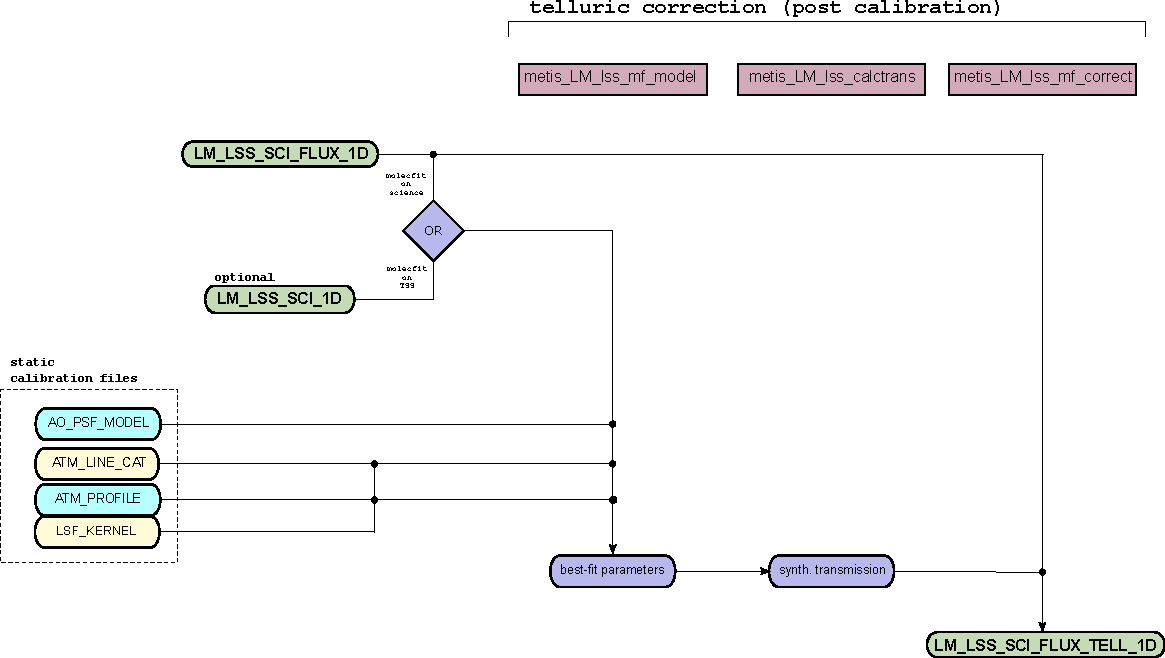
\includegraphics{figures/LM_LSS_pipeline_wf_draft_latest_part_2_v0.83.pdf}
  \caption[Reduction cascade and association map for LM long-slit
  spectroscopy]{Part 2 of the reduction cascade and association map for long-slit
    spectroscopy in the LM bands.}
  \label{Fig:LMLssAssomap2}
\end{figure}
\end{landscape}


% \begin{sidewaysfigure}[ht]
%   \centering
%   \includegraphics[width=0.9\textheight]{figures/NQ_LSS_pipeline_wf_draft_latest.png}
%   \caption[Reduction cascade and association map for N long-slit
%   spectroscopy]{Reduction cascade and association map for long-slit
%     spectroscopy in the N band.  }
%   \label{Fig:NQLssAssomap}
% \end{sidewaysfigure}


%% ---- Table: LM long-slit spectroscopy
%\begin{landscape}
%\begin{table}
%  \footnotesize
%  \begin{center}
%    \caption[Data Processing table for LM LSS: Main calibration]{%
%      Data Processing table for LM long-slit spectroscopy (cf. Fig.~\ref{Fig:LMLssAssomap1}): Main calibration}\bigskip
%    \label{Tab:LMLssDatProc1}
%    \begin{tabular}{|l|l|l|l|l|l|}
%      \hline
%      Data Type   & Classification & Recipe (Level)	& FITS Keywords & static/external  & Products\\
%    (Templates) & Keywords	 & Processing steps	&		&	CalibDB  &	\\
%    \hline
%    \TPL{DARK}	& \CODE{DPR.CATG==CALIB} & \hyperref[sssec:metis_det_dark]{\REC{metis_det_dark}} & Exposure time	&	\hyperref[dataitem:persistence_map]{\EXTCALIB{PERSISTENCE_MAP}} & Averaged dark frame\\
%    		& \CODE{DPR.TYPE==DARK}  &			&		&	\hyperref[dataitem:gain_map_2rg]{\PROD{GAIN_MAP_2RG}} & Bad pixel map\\
%    		& \CODE{DPR.TECH==IMAGE}  &			&		&	\hyperref[dataitem:linearity_2rg]{\PROD{LINEARITY_2RG}} & \\
%    \hline
%    \TPL{FLAT}	& \CODE{DPR.CATG==CALIB} & \hyperref[rec:metis_lm_lss_rsrf]{\REC{metis_LM_lss_rsrf}} & Exposure time	& \hyperref[dataitem:persistence_map]{\EXTCALIB{PERSISTENCE_MAP}}	& Averaged, normalized flatfield\\
%    		& \CODE{DPR.TYPE==FLAT}  &			&	Grism	& 	\hyperref[dataitem:gain_map_2rg]{\PROD{GAIN_MAP_2RG}} & \\
%    		& \CODE{DPR.TECH==SPECTRUM}  &			&	Slit	&	\hyperref[dataitem:linearity_2rg]{\PROD{LINEARITY_2RG}} & \\
%    \hline
%         	& \CODE{DPR.CATG==CALIB} &\hyperref[rec:metis_lm_lss_trace]{\REC{metis_LM_lss_trace}} & Exposure time	&	\hyperref[dataitem:persistence_map]{\EXTCALIB{PERSISTENCE_MAP}}& Order location\\
%    		& \CODE{DPR.TYPE==FLAT}  &			&		&	 \hyperref[dataitem:gain_map_2rg]{\PROD{GAIN_MAP_2RG}}& (polynomial fit)\\
%    		& \CODE{DPR.TECH==SPECTRUM}  &			&		&	\hyperref[dataitem:linearity_2rg]{\PROD{LINEARITY_2RG}} & \\
%    \hline
%    \TPL{WAVE,LASER} & \CODE{DPR.CATG==CATG} &\hyperref[rec:metis_lm_lss_wave]{\REC{metis_LM_lss_wave}} & Exposure time & \hyperref[dataitem:persistence_map]{\EXTCALIB{PERSISTENCE_MAP}}  & wavelength solution\\
%    		& \CODE{DPR.TYPE==WAVE,LASER}   &			   & Grism & \hyperref[dataitem:gain_map_2rg]{\PROD{GAIN_MAP_2RG}} &\\
%    		& \CODE{DPR.TECH==SPECTRUM}  &			& Slit		&	\hyperref[dataitem:linearity_2rg]{\PROD{LINEARITY_2RG}}& \\
%    		& \CODE{PRO.CATG==SPECTRUM}   &  &  & \hyperref[dataitem:laser_tab]{\STATCALIB{LASER_TAB}} & \\
%    \hline
%    \TPL{STD} & \CODE{DPR.CATG==CALIB} & \hyperref[rec:metis_lm_lss_std]{\REC{metis_LM_lss_std}}& Object name (\ac{STD} star) & \hyperref[dataitem:persistence_map]{\EXTCALIB{PERSISTENCE_MAP}} & Instrumental\\
%      & \CODE{DPR.TYPE==FLUX,STD}   &			   & Exposure time & \hyperref[dataitem:gain_map_2rg]{\PROD{GAIN_MAP_2RG}} & response function\\
%    		& \CODE{DPR.TECH==SPECTRUM}  &			&	Grism	&	\hyperref[dataitem:linearity_2rg]{\PROD{LINEARITY_2RG}} & Transmission (optionally)\\
%    		& \CODE{PRO.CATG==SPECTRUM}   &  & Slit & \hyperref[dataitem:atm_line_cat]{\EXTCALIB{ATM_LINE_CAT}} & Wavelength correction \\
%    		& & & & \hyperref[dataitem:lm_synth_trans]{\STATCALIB{LM_SYNTH_TRANS}} & (optionally)\\  
%    		& & & & \hyperref[dataitem:lm_adc_slitloss]{\STATCALIB{LM_ADC_SLITLOSS}} &\\    
%    		& & & &  \hyperref[dataitem:ao_psf_model]{\EXTCALIB{AO_PSF_MODEL}} &\\    
%%    		& & & & \hyperref[dataitem:tss_cont_tab]{\STATCALIB{TSS_CONT_TAB}} &\\    
%    		& & & & \hyperref[dataitem:ref_std_cat]{\STATCALIB{REF_STD_CAT}} &\\    \hline
%    \TPL{SCIENCE} & \CODE{DPR.CATG==SCIENCE} & \hyperref[rec:metis_lm_lss_sci]{\REC{metis_LM_lss_sci}} & Object name & \hyperref[dataitem:persistence_map]{\EXTCALIB{PERSISTENCE_MAP}}  & Science grade spectrum\\
%    		& \CODE{DPR.TYPE==OBJECT}   &			   & Exposure time & \hyperref[dataitem:gain_map_2rg]{\PROD{GAIN_MAP_2RG}} &\\
%    		& \CODE{DPR.TECH==SPECTRUM}  &			&	Grism	&\hyperref[dataitem:lm_adc_slitloss]{\STATCALIB{LM_ADC_SLITLOSS}} & \\
%    		& \CODE{PRO.CATG==SPECTRUM}   &  & Slit  &  \hyperref[dataitem:atm_line_cat]{\EXTCALIB{ATM_LINE_CAT}}	& \\
%    \hline
%    \end{tabular}
%  \end{center}
%\end{table}
%\end{landscape}
%\begin{landscape}
%\begin{table}
%  \footnotesize
%  \begin{center}
%    \caption[Data Processing table for LM LSS: Post-calibration / telluric correction]{%
%      Data Processing table for LM long-slit spectroscopy (cf. Fig.~\ref{Fig:LMLssAssomap2}): Post-calibration / telluric correction with \texttt{molecfit}}\bigskip
%    \label{Tab:LMLssDatProc2}
%    \begin{tabular}{|l|l|l|l|l|l|}  
%    \hline
%      Input   & Classification & Recipe (Level)	& FITS Keywords & static/external & Products\\
%    data & Keywords	 & Processing steps	&		&	 CalibDB  &	\\
%    \hline    
%%            Science grade spectrum & \CODE{DPR.CATG==SCIENCE} & \hyperref[rec:metis_lm_lss_mf_model]{\REC{metis_LM_lss_mf_model}} & Object name & \hyperref[dataitem:lsf_kernel]{\STATCALIB{LSF_KERNEL}}	 & Best-fit \\
%    		processed \ac{STD} spectrum& \CODE{DPR.TYPE==OBJECT}   &			  & & \hyperref[dataitem:atm_profile]{\EXTCALIB{ATM_PROFILE}}  & \texttt{molecfit} parameters\\
%    		& \CODE{DPR.TECH==TBD}  &			&		& \hyperref[dataitem:atm_line_cat]{\EXTCALIB{ATM_LINE_CAT}}	& \\
%    		& \CODE{PRO.CATG==TBD}   &  &  & start parameter set & \\
%    \hline
%            & \CODE{DPR.CATG==SCIENCE} &  \hyperref[rec:metis_lm_lss_mf_calctrans]{\REC{metis_LM_lss_mf_calctrans}} & Object name & \hyperref[dataitem:atm_line_cat]{\EXTCALIB{ATM_LINE_CAT}}	 & synthetic \\
%    		& \CODE{DPR.TYPE==LSS}   &		&	   &   & Transmission curve\\
%    		& \CODE{DPR.TECH==TBD}  &			&		& 	& \\
%    		& \CODE{PRO.CATG==TBD}   &  &  & & \\
%    \hline
%            & \CODE{DPR.CATG==SCIENCE} &  \hyperref[rec:metis_lm_lss_mf_correct]{\REC{metis_LM_lss_mf_correct}} & Object name &  & Absorption corrected\\
%    		& \CODE{DPR.TYPE==LSS}   &			   & &    & science spectrum\\
%    		& \CODE{DPR.TECH==TBD}  &			&		&	& \\
%    		& \CODE{PRO.CATG==TBD}   &  &  & & \\
%    \hline
%    \end{tabular}
%  \end{center}
%\end{table}
%\end{landscape}

\begin{landscape}
\begin{figure}[ht]
  \centering
  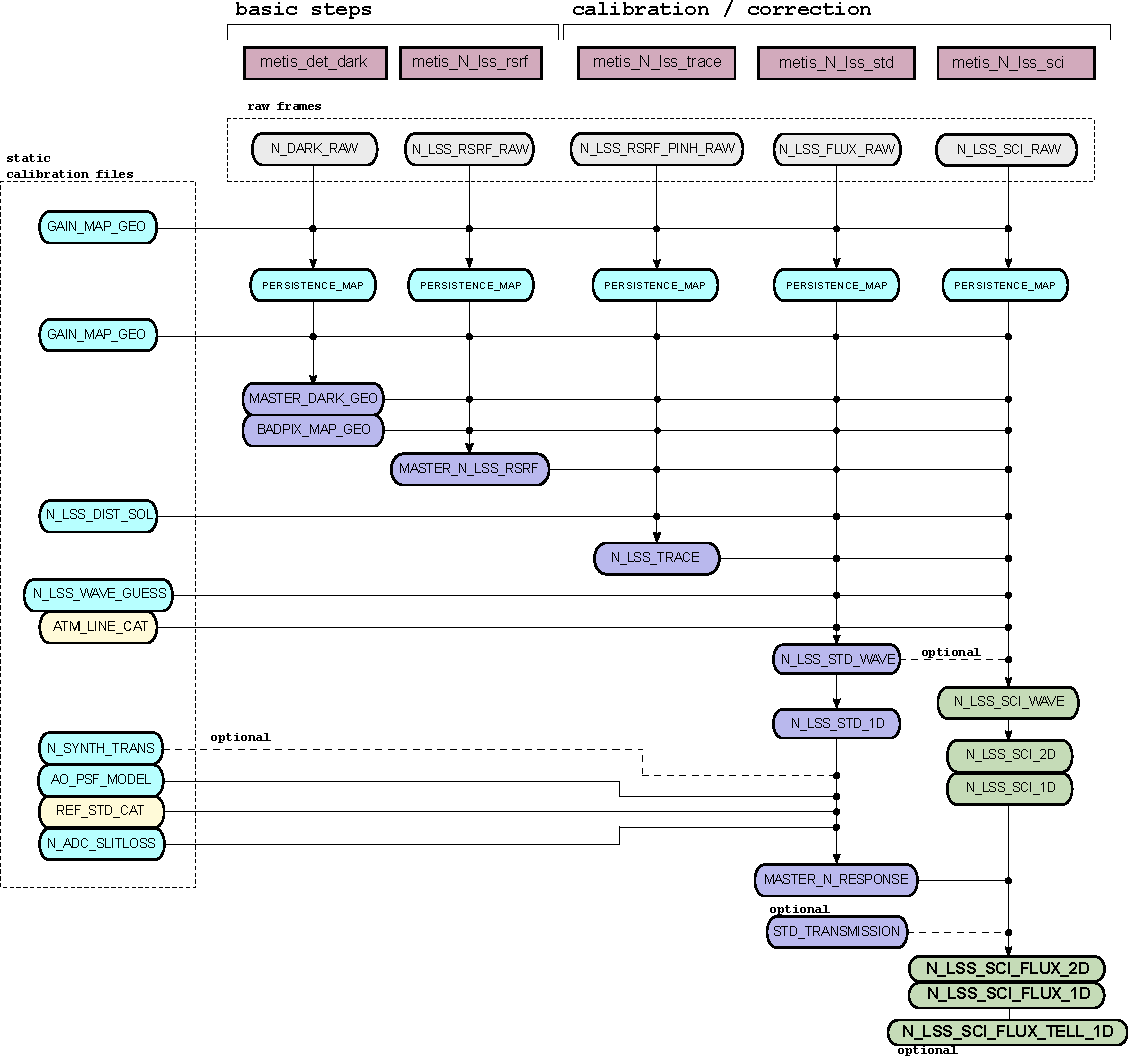
\includegraphics{figures/N_LSS_pipeline_wf_draft_latest_part_1_v0.83.pdf}
  \caption[Reduction cascade and association map for N long-slit
  spectroscopy]{Reduction cascade and association map for long-slit
    spectroscopy in the N bands. }
  \label{Fig:NLssAssomap1}
    \end{figure}
\end{landscape}

\begin{landscape}
\begin{figure}[ht]
  \centering
  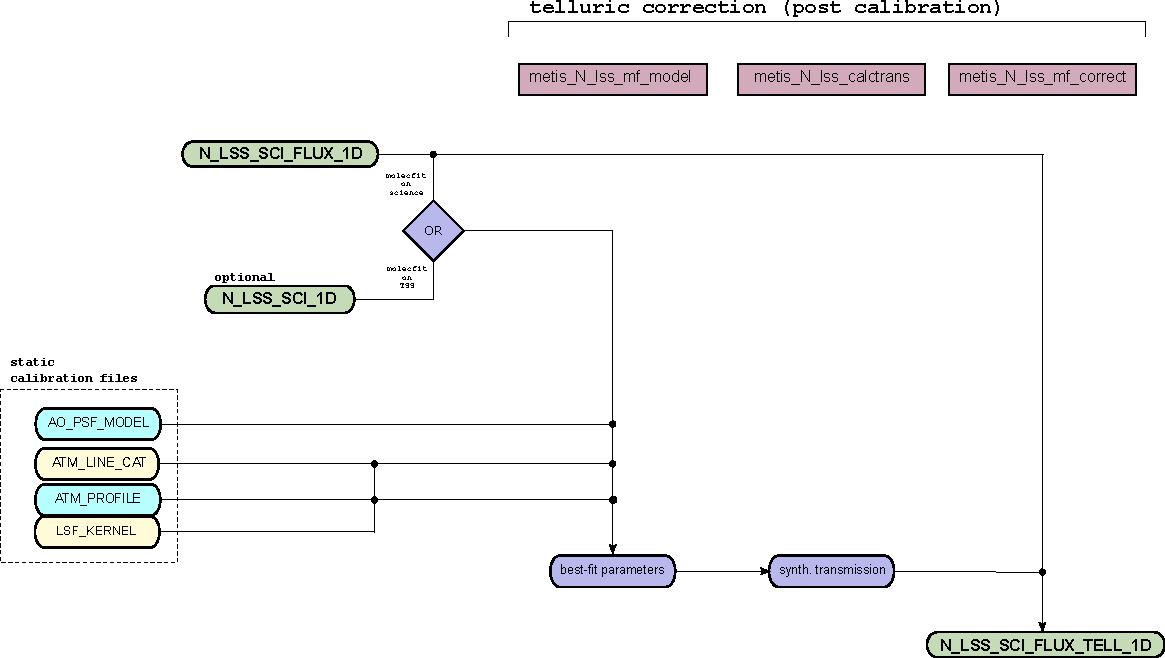
\includegraphics{figures/N_LSS_pipeline_wf_draft_latest_part_2_v0.83.pdf}
  \caption[Reduction cascade and association map for N long-slit
  spectroscopy]{Reduction cascade and association map for long-slit
    spectroscopy in the N bands. }
  \label{Fig:NLssAssomap2}
\end{figure}
\end{landscape}

%%% ---- Table: N long-slit spectroscopy
%\begin{landscape}
%\begin{table}
%  \footnotesize
%  \begin{center}
%    \caption[Data Processing table for N LSS: Main calibration]{%
%      Data Processing table for N long-slit spectroscopy (cf. Fig.~\ref{Fig:NLssAssomap1}): Main calibration}\bigskip
%    \label{Tab:NLssDatProc1}
%    \begin{tabular}{|l|l|l|l|l|l|}
%      \hline
%      Data Type   & Classification & Recipe (Level)	& FITS Keywords & static/external  & Products\\
%    (Templates) & Keywords	 & Processing steps	&		&	CalibDB  &	\\
%    \hline
%    \TPL{DARK}	& \CODE{DPR.CATG==CALIB} & \hyperref[sssec:metis_det_dark]{\REC{metis_det_dark}} & Exposure time	& 	\hyperref[dataitem:persistence_map]{\EXTCALIB{PERSISTENCE_MAP}} & Averaged dark frame\\
%    		& \CODE{DPR.TYPE==DARK}  &			&		&	\hyperref[dataitem:gain_map_geo]{\PROD{GAIN_MAP_GEO}} & Bad pixel map\\
%    		& \CODE{DPR.TECH==IMAGE}  &			&		&	\hyperref[dataitem:linearity_geo]{\PROD{LINEARITY_GEO}} & \\
%    \hline
%    \TPL{FLAT}	& \CODE{DPR.CATG==CALIB} & \hyperref[rec:metis_n_lss_rsrf]{\REC{metis_N_lss_rsrf}} & Exposure time	& \hyperref[dataitem:persistence_map]{\EXTCALIB{PERSISTENCE_MAP}}	& Averaged, normalized flatfield (\ac{RSRF}\\
%    		& \CODE{DPR.TYPE==FLAT}  &			&	Grism	&	\hyperref[dataitem:gain_map_geo]{\PROD{GAIN_MAP_GEO}} & Bad pixel map\\
%    		& \CODE{DPR.TECH==SPECTRUM}  &			& Slit		&	\hyperref[dataitem:linearity_geo]{\PROD{LINEARITY_GEO}} & \\
%    \hline
%         	& \CODE{DPR.CATG==CALIB} & \hyperref[rec:metis_n_lss_trace]{\REC{metis_N_lss_trace} }& Exposure time	& 	\hyperref[dataitem:persistence_map]{\EXTCALIB{PERSISTENCE_MAP}} & Order location\\
%    		& \CODE{DPR.TYPE==FLAT}  &			&	Grism	&	\hyperref[dataitem:gain_map_geo]{\PROD{GAIN_MAP_GEO}} & (polynomial fit)\\
%    		& \CODE{DPR.TECH==SPECTRUM}  &			&	Slit	&	 \hyperref[dataitem:linearity_geo]{\PROD{LINEARITY_GEO}} & \\
%    \hline
%    \TPL{STD} & \CODE{DPR.CATG==CALIB} & \hyperref[rec:metis_n_lss_std]{\REC{metis_N_lss_std}} & Object name (\ac{STD} star) & \hyperref[dataitem:persistence_map]{\EXTCALIB{PERSISTENCE_MAP}} & Instrumental\\
%    		& \CODE{DPR.TYPE==FLUX,STD}   &			   & Exposure time & \hyperref[dataitem:gain_map_geo]{\PROD{GAIN_MAP_GEO}} & response function\\
%    		& \CODE{DPR.TECH==SPECTRUM}   &			   & Grism		& \hyperref[dataitem:linearity_geo]{\PROD{LINEARITY_GEO}} & transmission (optional)\\
%    		& \CODE{PRO.CATG==SPECTRUM}   &  &  Slit & \hyperref[dataitem:n_lss_wave_guess]{\STATCALIB{N_LSS_WAVE_GUESS}} & wavelength correction\\
%    		& & & & \hyperref[dataitem:n_synth_trans]{\STATCALIB{N_SYNTH_TRANS}} &\\    		& & & &  \hyperref[dataitem:n_adc_slitloss]{\STATCALIB{N_ADC_SLITLOSS}} &\\
%    		& & & & \hyperref[dataitem:ao_psf_model]{\EXTCALIB{AO_PSF_MODEL}} &\\
%    		& & & & \hyperref[dataitem:n_lss_dist_sol]{\STATCALIB{N_LSS_DIST_SOL}} &\\
%   		& & & & \hyperref[dataitem:ref_std_cat]{\STATCALIB{REF_STD_CAT}} &\\
%    \hline
%    \TPL{SCIENCE} & \CODE{DPR.CATG==SCIENCE} & \hyperref[rec:metis_n_lss_sci]{\REC{metis_N_lss_sci}} & Object name &  \hyperref[dataitem:persistence_map]{\EXTCALIB{PERSISTENCE_MAP}} & Science grade spectrum\\
%    		& \CODE{DPR.TYPE==OBJECT}   &			   & Exposure time & \hyperref[dataitem:gain_map_geo]{\PROD{GAIN_MAP_GEO}}  &\\
%    		& \CODE{DPR.TECH==SPECTRUM}  &			&	Grism	&	\hyperref[dataitem:linearity_geo]{\PROD{LINEARITY_GEO}} & \\
%    		& \CODE{PRO.CATG==SPECTRUM}   &  & Slit & \hyperref[dataitem:atm_line_cat]{\EXTCALIB{ATM_LINE_CAT}}  & \\
%    		& & & & \hyperref[dataitem:n_adc_slitloss]{\STATCALIB{N_ADC_SLITLOSS}} &\\
%    		& & & & \hyperref[dataitem:n_lss_wave_guess]{\STATCALIB{N_LSS_WAVE_GUESS}} &\\
%    		& & & & \hyperref[dataitem:n_lss_dist_sol]{\STATCALIB{N_LSS_DIST_SOL}} &\\
%    \hline
%    \end{tabular}
%  \end{center}
%\end{table}

            
%\begin{table}
%  \footnotesize
%  \begin{center}
%    \caption[Data Processing table for N LSS: Post-calibration / telluric correction]{%
%      Data Processing table for N long-slit spectroscopy (cf. Fig.~\ref{Fig:NLssAssomap2}): Post-calibration / telluric correction with \texttt{molecfit} }\bigskip
%    \label{Tab:NLssDatProc2}
%    \begin{tabular}{|l|l|l|l|l|l|}
%      \hline
%      Input   & Classification & Recipe (Level)	& FITS Keywords & static/external & Products\\
%    data & Keywords	 & Processing steps	&		&	CalibDB  &	\\
%    \hline
%    Science grade spectrum & \CODE{DPR.CATG==SCIENCE} & \hyperref[rec:metis_n_lss_mf_model]{\REC{metis_N_lss_mf_model}} & Object name & \hyperref[dataitem:lsf_kernel]{\STATCALIB{LSF_KERNEL}}	 & Best-fit \\
%    	\ac{STD} star spectrum	& \CODE{DPR.TYPE==OBJECT}   &			  & & \hyperref[dataitem:atm_profile]{\EXTCALIB{ATM_PROFILE}}  & \texttt{molecfit} parameters\\
%    		& \CODE{DPR.TECH==TBD}  &			&		& \hyperref[dataitem:atm_line_cat]{\EXTCALIB{ATM_LINE_CAT}}	& \\
%    		& \CODE{PRO.CATG==TBD}   &  &  & start parameter set & \\
%    \hline
%            & \CODE{DPR.CATG==SCIENCE} & \hyperref[rec:metis_n_lss_mf_calctrans]{\REC{metis_N_lss_mf_calctrans}} & Object name & \hyperref[dataitem:atm_line_cat]{\EXTCALIB{ATM_LINE_CAT}}	 & synthetic \\
%    		& \CODE{DPR.TYPE==LSS}   &		&	   &  & Transmission curve\\
%    		& \CODE{DPR.TECH==TBD}  &			&		&  	& \\
%    		& \CODE{PRO.CATG==TBD}   &  &  & & \\
%    \hline
%            & \CODE{DPR.CATG==SCIENCE} & \hyperref[rec:metis_n_lss_mf_correct]{\REC{metis_N_lss_mf_correct}} & Object name &  & Absorption corrected\\
%    		& \CODE{DPR.TYPE==LSS}   &			   &  & & science spectrum\\
%    		& \CODE{DPR.TECH==TBD}  &			&		&	& \\
%    		& \CODE{PRO.CATG==TBD}   &  &  & & \\
%    \hline
%    \end{tabular}
%  \end{center}
%\end{table}
%\end{landscape}

\restoregeometry

\subsubsection{Static calibration database}\label{lss:static_calib}
The static calibration database comprises several data sets, some are updated from time to time:
\begin{itemize}
    \item \hyperref[dataitem:gain_map_2rg]{\PROD{GAIN_MAP_2RG}}, \hyperref[dataitem:gain_map_geo]{\PROD{GAIN_MAP_GEO}}: These are the detector gain maps of the detectors (2RG=Hawaii2RG, LM-band; GEO=Geosnap, N-band), which are created by the recipe \hyperref[sssec:metis_det_lingain]{\REC{metis_det_lingain}} (see Section~\ref{sssec:metis_det_lingain}). This recipe is carried out every once in a while (yearly, TBD, see \cite{METIS-calibration_plan}) as we assume the detectors to be fairly stable.
    \item \hyperref[dataitem:linearity_2rg]{\PROD{LINEARITY_2RG}}, \hyperref[dataitem:linearity_geo]{\PROD{LINEARITY_GEO}}: These are the coefficients for the correction of the linearity of the individual pixels. Also created by the recipe \hyperref[sssec:metis_det_lingain]{\REC{metis_det_lingain}} (see Section~\ref{sssec:metis_det_lingain}). 
    \item \hyperref[dataitem:laser_tab]{\STATCALIB{LASER_TAB}}: The \ac{WCU} provides laser sources for the first guess of the wavelength solution. The main laser frequencies are fixed (\cite{METIS-calibration_plan}) and given in a static table.
    \item \hyperref[dataitem:atm_line_cat]{\EXTCALIB{ATM_LINE_CAT}}: The main wavelength calibration will be done by means of atmospheric lines, most probably based on the \ac{HITRAN}\footnote{\url{https://hitran.org/}}. They are given in a static catalogue. This database is also required by the telluric correction package \texttt{molecfit}.
    \item \hyperref[dataitem:lm_synth_trans]{\STATCALIB{LM_SYNTH_TRANS}}/\hyperref[dataitem:n_synth_trans]{\STATCALIB{N_SYNTH_TRANS}}: For the determination of the continuum of flux standard stars a rough telluric correction is needed. We intend to also offer the possibility to apply static transmission curves for that purpose for performance reasons. These static transmission curves will be determined during commissioning via \texttt{molecfit} or by means of the ESO SkyCalc Tool\footnote{\url{https://www.eso.org/observing/etc/bin/gen/form?INS.MODE=swspectr+INS.NAME=SKYCALC}}.
    \item \hyperref[dataitem:ao_psf_model]{\EXTCALIB{AO_PSF_MODEL}}: Due to the broad wings of the \ac{PSF} there might be a fraction of the flux falling outside the long slits, leading to some losses. Depending on the stability of the \ac{AO} performance, these losses might be non-constant and maybe need some correction by estimating width of the \ac{PSF}. One idea is to incorporate a static \ac{PSF} model, which is scaled by some \ac{AO} telemetry data. However, many details on that topic are still unclear and remain TBD. We therefore keep it as placeholder for the time being until it is clarified whether such a correction is necessary.
    \item \hyperref[dataitem:ref_std_cat]{\STATCALIB{REF_STD_CAT}}: Catalogue of standard stars used for the absolute flux calibration and (optionally) the telluric correction. This catalogue contains theoretical models of a set of standard stars (cf. Section~\ref{ssec:tellcorr}). 
    %\item \hyperref[dataitem:tss_model_cat]{\STATCALIB{TSS_MODEL_CAT}}: In some cases, the default modelling method for the telluric correction might not be possible or leading to bad results. We therefore foresee the possibility to use telluric standard stars. For the determination of the transmisison function a model of the selected telluric star is required to remove intrinisic stellar features. In this table, models of a set of such stars are provided to be used for that purpose.
    %\item \hyperref[dataitem:tss_cont_tab]{\STATCALIB{TSS_CONT_TAB}}: Spectra of telluric standard stars need to be normalised to derive the transmission function of the Earth's atmosphere out of them. This normalisation is done by a polynomial fit on stellar regions unaffected by intrinsic or atmospheric features, ddepend also on the type of the selected star. This table provides continuum regions of the telluric standard star set.
    \item \hyperref[dataitem:lm_adc_slitloss]{\STATCALIB{LM_ADC_SLITLOSS}}/\hyperref[dataitem:n_adc_slitloss]{\STATCALIB{N_ADC_SLITLOSS}}: It is expected that the fixed positions of the \ac{ADC} will introduce specific slit losses. These losses are determined in the recipes \hyperref[rec:metis_lm_adc_slitloss]{\REC{metis_lm_adc_slitloss}} and \hyperref[rec:metis_n_adc_slitloss]{\REC{metis_n_adc_slitloss}} (see Section~\ref{sssec:adc_slitlosses} and \cite{METIS-calibration_plan}). As these losses are assumed to be very stable, these recipes will be carried out only rarely.
    \item \hyperref[dataitem:atm_profile]{\EXTCALIB{ATM_PROFILE}} and \hyperref[dataitem:lsf_kernel]{\STATCALIB{LSF_KERNEL}}: The telluric correction package \texttt{molecfit} requires an atmospheric profile incorporating height information of the temperature, pressure and molecular abundances as input. Currently we use a static profile (equatorial \texttt{equ.atm}\footnote{\url{https://eodg.atm.ox.ac.uk/RFM/atm/}}) as starting point of the fit of the molecular column densities. In addition, a kernel for the \ac{LSF} is provided. We intend to determine the kernel during commissioning and use this as input. However, it is still unclear in how far the \ac{AO} influences that kernel. The current baseline is to use the static \hyperref[dataitem:lsf_kernel]{\STATCALIB{LSF_KERNEL}} as starting point for fitting the line spread function.
    \item \hyperref[dataitem:n_lss_dist_sol]{\STATCALIB{N_LSS_DIST_SOL}}/\hyperref[dataitem:n_lss_wave_guess]{\STATCALIB{N_LSS_WAVE_GUESS}}: First guess solutions of the N-band LSS mode are static due to the absence of laser sources after \ac{AIT}. As the instrument is expected to be very stable, these calibration files will be created only once and kept static.
\end{itemize}
